\documentclass[12pt]{article}
\usepackage{amsmath}
\usepackage{tikz}
\usetikzlibrary{automata, positioning, arrows}
\tikzset{->, >=stealth, node distance=3cm, every state/.style={thick, fill=gray!10}, initial text=$ $,}
\renewcommand{\thesubsection}{\alph{subsection}.}

\title{CENG280 Homework 1}
\author{Murat Bolu}
\date{2521300}

\begin{document}

\maketitle

\section{Question 1}

\subsection{}
\begin{equation*}
((a \cup b)^*\ aa\ (a \cup b)^*\ bb\ (a \cup b)^*) \cup ((a \cup b)^*\ bb\ (a \cup b)^*\ aa\ (a \cup b)^*)
\end{equation*}

\subsection{}
\begin{center}
Formal definition of the nondeterministic finite automaton M:
\end{center}
\begin{align*}
M = (\{q_0,q_1,q_2,q_3,q_4,q_5,q_6,q_7\},\{a,b\}, \{&(q_0, a, q_0), (q_0, b, q_0), (q_0, a, q_1), (q_1, a, q_2), \\
&(q_2, a, q_2), (q_2, b, q_2), (q_2, b, q_3), (q_3, b, q_7), \\
&(q_0, b, q_4), (q_4, b, q_5), (q_5, a, q_5), (q_5, b, q_5), \\
&(q_5, a, q_6), (q_6, a, q_7), (q_7, a, q_7), (q_7, b, q_7)\}, q_0, \{q_7\})
\end{align*}

\newpage

\begin{center}
Drawing of the nondeterministic finite automaton M:
\end{center}

\begin{figure}[ht]
    \centering
    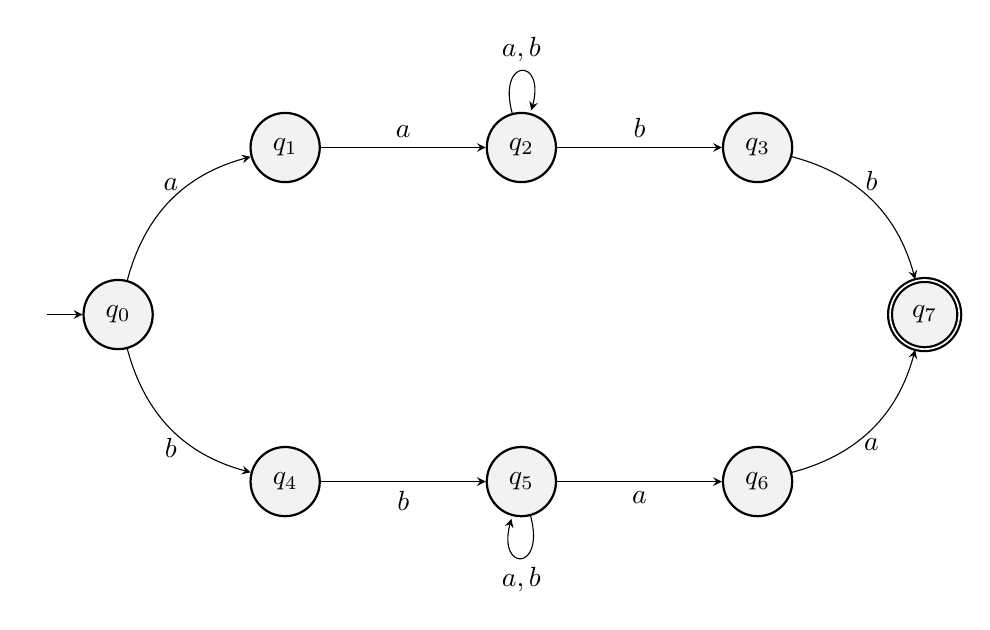
\begin{tikzpicture}
        \node[state, initial] (q0) {$q_0$};
        \node[state, above right of=q0] (q1) {$q_1$};
        \node[state, right of=q1] (q2) {$q_2$};
        \node[state, right of=q2] (q3) {$q_3$};
        \node[state, below right of=q0] (q4) {$q_4$};
        \node[state, right of=q4] (q5) {$q_5$};
        \node[state, right of=q5] (q6) {$q_6$};
        \node[state, accepting, below right of=q3] (q7) {$q_7$};
        
        \draw (q0) edge[bend left, above] node{$a$} (q1)
                  (q0) edge[bend right, below] node{$b$} (q4)
                  (q1) edge[above] node{$a$} (q2)
                  (q2) edge[loop above] node{$a,b$} (q2)
                  (q2) edge[above] node{$b$} (q3)
                  (q3) edge[bend left, above] node{$b$} (q7)
                  (q4) edge[below] node{$b$} (q5)
                  (q5) edge[loop below] node{$a,b$} (q5)
                  (q5) edge[below] node{$a$} (q6)
                  (q6) edge[bend right, below] node{$a$} (q7);
    \end{tikzpicture}
    \caption{Nondeterministic Finite Automaton M}
    \label{fig:nfa}
\end{figure}

\subsection{}

\begin{center}
Let's formally define the deterministic finite automaton $M'$, which will be equivalent to $M$.
We don't need to use $E(q_i)$ notation since there are no empty transitions in our NFA.
\end{center}
\begin{equation*}
M' = (K', \Sigma, \delta', s', F')
\end{equation*}
\begin{center}
Where $\Sigma = \{a, b\}$, same with the NFA. \\
Where $s' = \{q_0\}$, the set of all states that are reachable from the start state without reading any input. \\
\end{center}

\newpage

\begin{center}
We need to construct $\delta'$ by taking the set of start states, defining the transitions of it accordingly and defining transitions of the new states until all states are defined.
\end{center}

\begin{align*}
\text{Where \ } \delta'(\{q_0\}, a) &= \{q_0, q_1\} \\
\delta'(\{q_0\}, b) &= \{q_0, q_4\} \\
\delta'(\{q_0, q_1\}, a) &= \{q_0, q_1, q_2\} \\
\delta'(\{q_0, q_1\}, b) &= \{q_0, q_4\} \\
\delta'(\{q_0, q_4\}, a) &= \{q_0, q_1\} \\
\delta'(\{q_0, q_4\}, b) &= \{q_0, q_4, q_5\} \\
\delta'(\{q_0, q_1, q_2\}, a) &= \{q_0, q_1, q_2\} \\
\delta'(\{q_0, q_1, q_2\}, b) &= \{q_0, q_2, q_3, q_4\} \\
\delta'(\{q_0, q_4, q_5\}, a) &= \{q_0, q_1, q_5, q_6\} \\
\delta'(\{q_0, q_4, q_5\}, b) &= \{q_0, q_4, q_5\} \\
\delta'(\{q_0, q_2, q_3, q_4\}, a) &= \{q_0, q_1, q_2\} \\
\delta'(\{q_0, q_2, q_3, q_4\}, b) &= \{q_0, q_2, q_3, q_4, q_5, q_7\} \\
\delta'(\{q_0, q_1, q_5, q_6\}, a) &= \{q_0, q_1, q_2, q_5, q_6, q_7\} \\
\delta'(\{q_0, q_1, q_5, q_6\}, b) &= \{q_0, q_4, q_5\} \\
\delta'(\{q_0, q_2, q_3, q_4, q_5, q_7\}, a) &= \{q_0, q_1, q_2, q_5, q_6, q_7\} \\
\delta'(\{q_0, q_2, q_3, q_4, q_5, q_7\}, b) &= \{q_0, q_2, q_3, q_4, q_5, q_7\} \\
\delta'(\{q_0, q_1, q_2, q_5, q_6, q_7\}, a) &= \{q_0, q_1, q_2, q_5, q_6, q_7\} \\
\delta'(\{q_0, q_1, q_2, q_5, q_6, q_7\}, b) &= \{q_0, q_2, q_3, q_4, q_5, q_7\} \\
\end{align*}
\begin{align*}
\text{Where } K' = \{\{q_0\}, \{q_0, q_1\}, \{q_0, q_4\}, \{q_0, q_1, q_2\}, \\
\{q_0, q_4, q_5\}, \{q_0, q_2, q_3, q_4\}, \{q_0, q_1, q_5, q_6\}, \\
\{q_0, q_2, q_3, q_4, q_5, q_7\}, \{q_0, q_1, q_2, q_5, q_6, q_7\}\} \text{,} \\
\text{the set of all possible sets of states.} \\
\end{align*}
\begin{align*}
&\text{Where } F' = \{\{q_0, q_2, q_3, q_4, q_5, q_7\}, \{q_0, q_1, q_2, q_5, q_6, q_7\}\} \text{,} \\
&\text{the set of all sets in $K'$ containing a common element with $s'$.}
\end{align*}

\newpage

\begin{center}
Drawing of the deterministic finite automaton M':
\end{center}

\begin{figure}[ht]
    \centering
    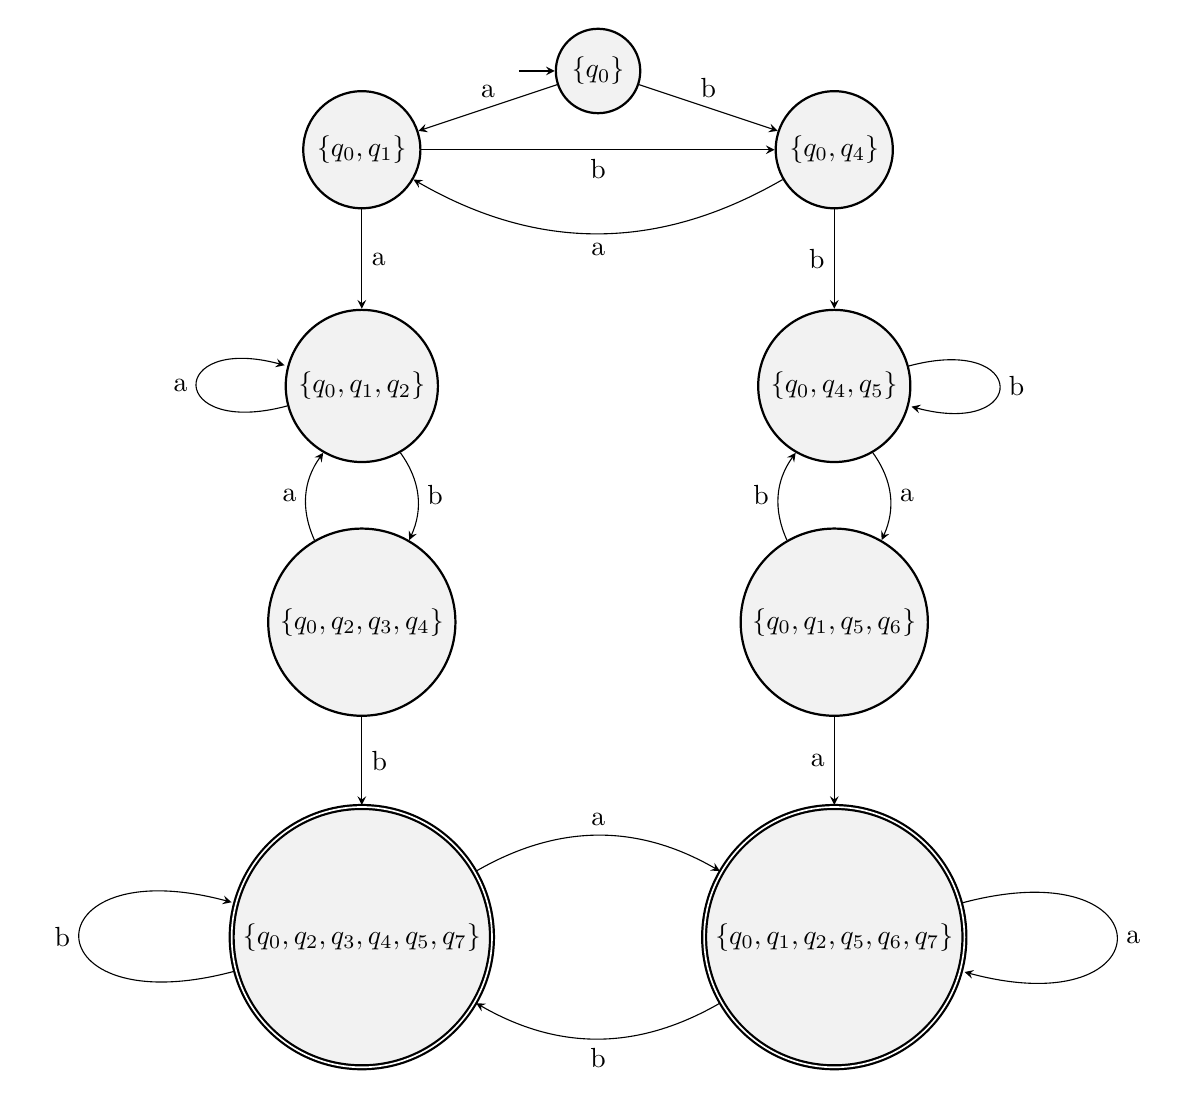
\begin{tikzpicture}
        \node[state, initial] at (5,0) (q0) {$\{q_0\}$};
        \node[state] at (2,-1) (q0q1) {$\{q_0, q_1\}$};
        \node[state] at (8,-1) (q0q4) {$\{q_0, q_4\}$};
        \node[state] at (2, -4) (q0q1q2) {$\{q_0, q_1, q_2\}$};
        \node[state] at (8,-4) (q0q4q5) {$\{q_0, q_4, q_5\}$};
        \node[state] at (2, -7) (q0q2q3q4) {$\{q_0, q_2, q_3, q_4\}$};
        \node[state] at (8, -7) (q0q1q5q6) {$\{q_0, q_1, q_5, q_6\}$};
        \node[state, accepting] at (2, -11) (q0q2q3q4q5q7) {$\{q_0, q_2, q_3, q_4, q_5, q_7\}$};
        \node[state, accepting] at (8, -11) (q0q1q2q5q6q7) {$\{q_0, q_1, q_2, q_5, q_6, q_7\}$};
        
        \draw (q0) edge[above] node{a} (q0q1)
                  (q0) edge[above] node{b} (q0q4)
                  (q0q1) edge[right] node{a} (q0q1q2)
                  (q0q1) edge[below] node{b} (q0q4)
                  (q0q4) edge[bend left, below] node{a} (q0q1)
                  (q0q4) edge[left] node{b} (q0q4q5)
                  (q0q1q2) edge[loop left] node{a} (q0q1q2)
                  (q0q1q2) edge[bend left, right] node{b} (q0q2q3q4)
                  (q0q4q5) edge[bend left, right] node{a} (q0q1q5q6)
                  (q0q4q5) edge[loop right] node{b} (q0q4q5)
                  (q0q2q3q4) edge[bend left, left] node{a} (q0q1q2)
                  (q0q2q3q4) edge[right] node{b} (q0q2q3q4q5q7)
                  (q0q1q5q6) edge[left] node{a} (q0q1q2q5q6q7)
                  (q0q1q5q6) edge[bend left, left] node{b} (q0q4q5)
                  (q0q2q3q4q5q7) edge[bend left, above] node{a} (q0q1q2q5q6q7)
                  (q0q2q3q4q5q7) edge[loop left] node{b} (q0q2q3q4q5q7)
                  (q0q1q2q5q6q7) edge[loop right] node{a} (q0q1q2q5q6q7)
                  (q0q1q2q5q6q7) edge[bend left, below] node{b} (q0q2q3q4q5q7);
    \end{tikzpicture}
    \caption{Deterministic Finite Automaton M'}
    \label{fig:dfa}
\end{figure}

\newpage

\subsection{}

\begin{equation*}
\begin{split}
(\{q_0\}, bbabb) &\vdash_{M'} (\{q_0, q_4\}, babb) \\
&\vdash_{M'} (\{q_0, q_4, q_5\}, abb) \\
&\vdash_{M'} (\{q_0, q_1, q_5, q_5\}, bb) \\
&\vdash_{M'} (\{q_0, q_4, q_5\}, b) \\
&\vdash_{M'} (\{q_0, q_4, q_5\}, e) \\
\end{split}
\end{equation*}
\begin{center}
The string $"bbabb"$ is not accepted by the DFA $M'$ since $\{q_0, q_4, q_5\}$ is not an element of $F'$.
\end{center}

\begin{align*}
(q_0, bbabb) &\vdash_M (q_4, babb) & (q_0, bbabb) &\vdash_M (q_0, babb) \\
&\vdash_M (q_5, abb) & &\vdash_M (q_0, abb) \\
&\vdash_M (q_6, bb) & &\vdash_M (q_1, bb) \\
&\text{Machine halts.} & &\text{Machine halts.}  \\[5 pt]
(q_0, bbabb) &\vdash_M (q_0, babb) & (q_0, bbabb) &\vdash_M (q_4, babb)\\
&\vdash_M (q_0, abb) & &\vdash_M (q_5, abb) \\
&\vdash_M (q_0, bb) & &\vdash_M (q_5, bb) \\
&\vdash_M (q_0, b) & &\vdash_M (q_5, b) \\
&\vdash_M (q_0, e) & &\vdash_M (q_5, e) \\
&\text{Not accepted.} & &\text{Not accepted.}\\[5 pt]
(q_0, bbabb) &\vdash_M (q_0, babb) \\
&\vdash_M (q_0, abb) \\
&\vdash_M (q_0, bb) \\
&\vdash_M (q_4, b) \\
&\vdash_M (q_5, e) \\
&\text{Not accepted.} \\
\end{align*}
\begin{center}
This is not an exhaustive list but one can try every possible combination and see that $"bbabb"$ is not accepted by the NFA $M$.
\end{center}

\newpage

\section{Question 2}

\subsection{}

\begin{center}
Assume $L_2$ is regular.
That means $\overline{L_1}$ is also regular.
By closure property of complementation of regular languages, $\overline{L_2}$ is also regular.
Since $L_2 = \overline{L_1} \Rightarrow \overline{L_2}=\overline{\overline{L_1}} \Rightarrow \overline{L_2}=L_1,\ L_1$ is also regular.
This means that by pumping lemma, there is an integer $p \ge 1$ such that any string $w \in L_1$ with $\vert w\vert \ge p$ can be partitioned into $w=xyz$ where $y\neq e, \vert xy\vert \le p$, and $xy^iz \in L_1$ for all $i \ge 0$.
Let $w = a^{p+1}b^p \in L_1$.
Then $w$ can be written as $xyz$, where $y = a^j$ because of the $\vert xy\vert \leq p$ constraint and $1 \le j \le p$.
If we pump down the string by taking $i=0$ in $xy^iz$, the new string $w'$ becomes $w' = xz$.
Considering the fact that the number of $a$'s in the string was only one more than the number of $b$'s in the string, pumping down makes the number of $a$'s less than or equal to the number of $b$'s, which makes $w' \notin L1$.
This leads to a contradiction, therefore $L_2$ is not regular.
\end{center}

\subsection{}

\begin{center}
The subset of $L_5$ where $m=n$ and $m \neq 0$ and $n \neq 0$ is equivalent to $L_4$.
Therefore $L_4 \cup L_5 = L_5$ by set properties.
$L_5$ is regular since it is equivalent to the language of the regular expression $a^*b^*$.
$L_6$ is regular since it is a regular expression.
Therefore $L_4 \cup L_5 \cup L_6 = L_5 \cup L_6$ which is regular by closure property of union of regular languages.
\end{center}

\end{document}

